\chapter{V.E.C.T.O.R. -3000}

\begin{figure}[H]
    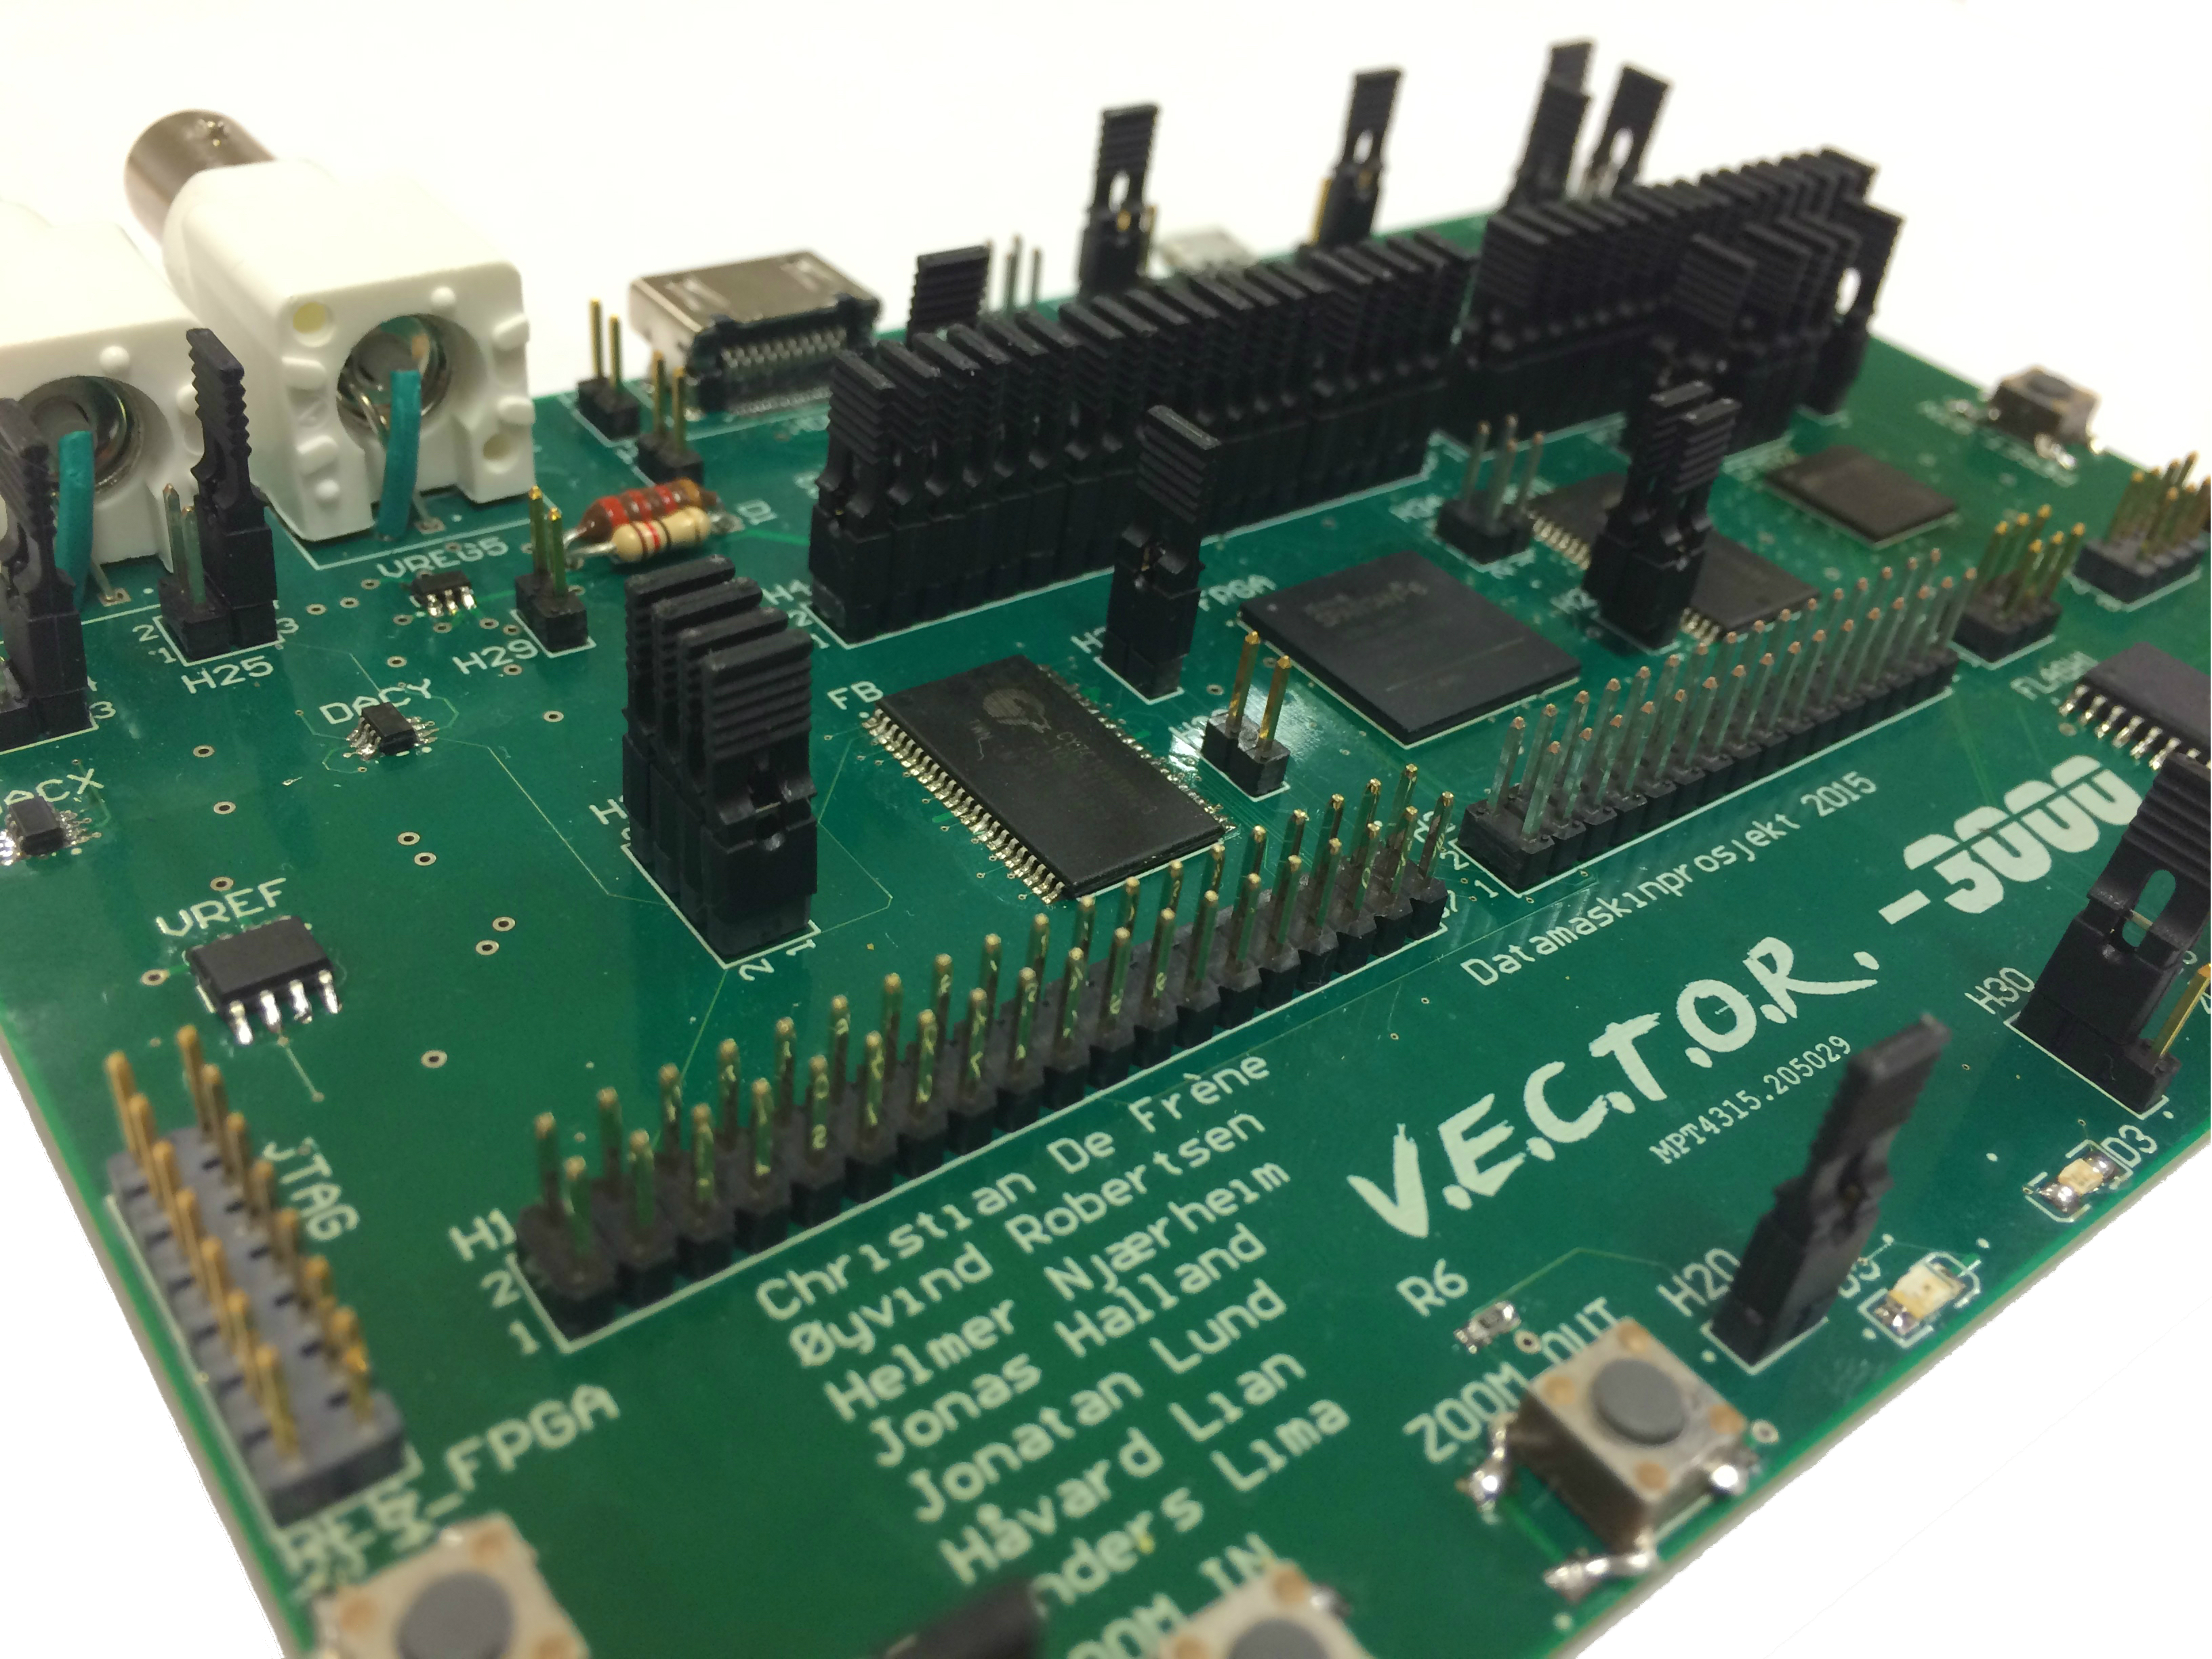
\includegraphics[width=\linewidth]{images/board_angle.jpg}
    \caption{V.E.C.T.O.R. -3000}
    \label{fig:board-angle}
\end{figure}

The end result of the group's work on this project is a computer architecture made with the defined requirements in mind.
The architecture is named V.E.C.T.O.R -3000, an acronym for Very Efficient Computer for Transferring graphics to Oscilloscope and Raster screens, with the -3000 added as an homage to the retrofuturistic associations of vector graphics in popular culture.

V.E.C.T.O.R. -3000 is a general purpose vector graphics processor, capable of processing and producing vector graphics. 
It utilizes a multi cycle processor core, an instruction level parallellism technique that benefits the processor by allowing shorter clock cycles.
This feature, together with the minimalistic instruction set architecture (ISA) inspired by RISC\cite{risc} and MIPS\cite{mips}, results in a computer that fits into today's computing world.
The vectorized output is sent to the oscilloscope, where it is displayed on the vector display in it's full glory.